%\documentclass[11pt,a4paper]{report}
\documentclass[11pt,a4paper]{article}
%\documentclass[11pt,a4paper]{amsart}

\usepackage{listings}
\usepackage{amsmath}
\usepackage{verbatim}
\usepackage{graphicx}
\usepackage[usenames,dvipsnames]{color}

\lstset{language=Python}

\title{Cylc: A Self-Organising Optimal Job Scheduler 
For Complex Environmental Forecasting Systems}

\author{Hilary Oliver, NIWA}

\begin{document}

\maketitle

\pagebreak
\tableofcontents
\pagebreak

\begin{abstract}

    {\em Cylc} is a self-organising metascheduler\footnote{A
    metascheduler sends dependent tasks to the batch queue job
    scheduler(s) when it has determined that they are {\em ready to
    run}. However, we drop the ``meta'' prefix from here on because a
    metascheduler is also a type of scheduler. The term
    ``metascheduler'' can also refer to a single aggregate view of
    multiple distributed resource managers, but that is not the topic of
    this paper.} for cycling environmental forecast systems comprising
    any number of linked scientific models and associated data
    collection, preprocessing, postprocessing, and product generation
    tasks.\footnote{A {\em task} is any group of processes treated as a
    single entity for scheduling purposes.} Its novel scheduling
    algorithm maintains an evolving pool of tasks from multiple forecast
    cycles\footnote{For our purposes a {\em forecast cycle} comprises
    all tasks with a common {\em forecast reference time}, which is the
    analysis time or nominal start time of a forecast model, or that of
    the associated forecast model(s) other tasks.} that interact to
    resolve dependencies.\footnote{Strictly speaking the task pool
    contains proxy objects that represent real tasks.} Each task is
    defined in isolation and knows its own prerequisites (but not who
    will satisfy them) and outputs (but not who will use them), and
    there is no need for a global ``suite'' definition that specifies
    dependencies or execution order.  If the external driving
    data\footnote{Forecast systems are typically driven by observational
    data and/or timely model fields from an external forecasting
    system.} for upcoming forecast cycles are available in advance {\em
    cylc} can run tasks from multiple cycles at once to the full extent
    allowed by intercycle dependencies; a series of distinct forecast
    cycles emerges only when the system catches up to real time
    operation.\footnote{{\em Cylc} also enables new modes of real time
    operation, for example a catchment river model that runs hourly
    assimilating real time stream flow observations and using the {\em
    most recent} 6-hourly precipitation forecast - see EcoConnect,
    below).} This means that parallel test systems can be started (or
    restarted) behind the main operation to catch up as quickly as
    possible, systems with little downtime between forecast cycles will
    catch up from delays much faster, and historical case studies can
    achieve sustained maximal throughput. {\em Cylc} is easily
    interfaced to existing tasks and is extremely flexible and easy to
    use. It can be restarted in arbitrarily complex states of operation
    and dynamically adapts to insertion or removal of tasks.  A failed
    task will necessarily delay its downstream dependants, but the rest
    of the system can carry on unaffected while the problem is
    addressed, after which time the delayed tasks will catch up as
    quickly as possible.  {\em Cylc}'s handling of forecast model
    `restart' dependencies allows continued operation, with very little
    operator intervention, over major failures that result in omitted
    forecast cycles in the driving (upstream) models.  Ability to
    control the configured task set, and failure recovery scenarios, can
    be completely tested in an accelerated simulation mode that is
    indistinguishable (to {\em cylc}) from real operation.  {\em Cylc}
    is written in object oriented Python and uses the Python Remote
    Object Protocol ({\em Pyro}) to control tasks across a network.  

\end{abstract}

\section{Forecasting Systems}
\label{sec:FS}

Environmental forecasting systems generate forecast products at regular
intervals using potentially large sets of scientific models and
associated data processing tasks. They are constrained by availability
of external driving data, typically real time observations and/or model
data from an external forecasting system, which one or more ``top
level'' tasks depend on; these drive other ``downstream'' task, and so
on. The dependency diagram for such a system consists of one or more
(possibly linked) {\em Directed Acyclic Graphs}, which may vary
according to ``forecast cycle'' (wherein each task has the same {\em
forecast reference time}, namely the nominal analysis time or start time
of the forecast models or, for data processing tasks, that of their
associated forecast model). Normal real time operation necessarily
consists of a series of distinct forecast cycles that are initiated,
after a gap in processing, by arrival of new external driving data.

From a job scheduling perspective the execution order of the various
tasks must be carefully controlled to avoid dependency violations.
Ideally, each task should be queued for execution at the instant its
last prerequisite is satisfied; this is the best that can be done even
if queued tasks are not able to execute immediately because of resource
contention.


\subsection{EcoConnect}

This work was motivated by the EcoConnect Forecasting System at NIWA
(National Institute of Water and Atmospheric Research, New Zealand).  As
of mid 2009, EcoConnect takes real time atmospheric and stream flow
observations, and operational global weather forecasts from the Met
Office (UK), and uses these to drive global sea state and regional data
assimilating weather models, which in turn drive regional sea state,
storm surge, and catchment river models, plus tide prediction, and a
large number of associated data collection, quality control,
preprocessing, postprocessing, product generation, and archiving
tasks.\footnote{Plans for EcoConnect include additional deterministic
regional weather forecasts and a statistical ensemble.} The global sea
state forecast runs once daily.  The regional weather forecast runs four
times daily but it supplies surface pressures to several downstream
models that run only twice daily, and precipitation accumulations to
catchment river models that run on an hourly cycle assimilating real
time stream flow observations and using the most recent available
regional weather forecast.  EcoConnect runs on heterogenous distributed
hardware, including a massively parallel supercomputer and several Linux
servers. 

\subsection{The Impact of Dependencies}

Most dependencies occur between tasks within a single forecast cycle. A
sea state forecast, for example, might depend on surface wind fields
generated by an upstream weather forecast over the same forecast range,
and a product generation task clearly cannot run before its associated
forecast model has generated output for it to process. Figure
\ref{fig-dep-one} shows the dependency diagram for a single forecast
cycle of a simple example system consisting of three forecast models
({\em a, b,} and {\em c}) and three post processing or product
generation tasks ({\em d, e} and {\em f}).  A scheduling system capable
of handling this must manage, within a single forecast cycle, multiple
parallel streams of execution that branch when one task generates output
for several downstream tasks, and merge when one task takes input from
several upstream tasks. 

\begin{figure} 
    \begin{center}
    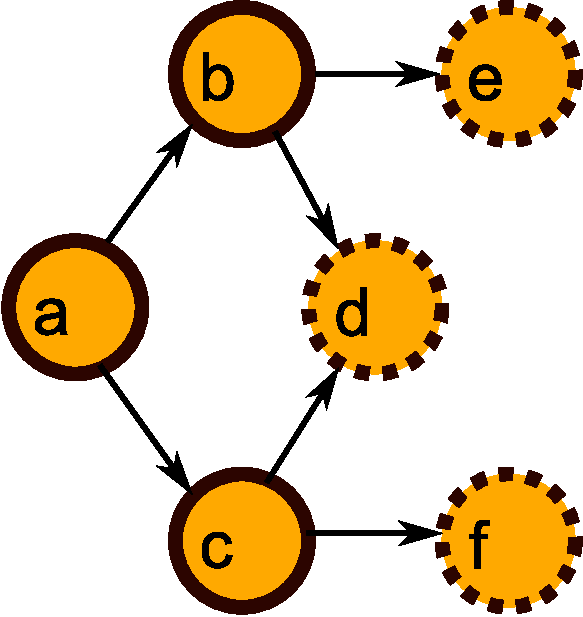
\includegraphics[width=4cm]{dependencies-one} 
    \end{center}
    \caption{\small Dependency diagram for a single forecast cycle in a
    simple example system. Tasks {\em a, b,} and {\em c} represent
    forecast models, and {\em d, e} and {\em f} are post processing or
    product generation tasks.} 
    \label{fig-dep-one} 
\end{figure} 

\begin{figure}
    \begin{center}
        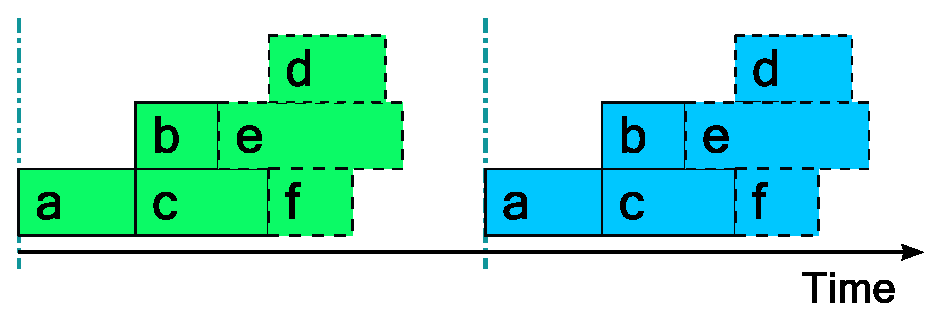
\includegraphics[width=8cm]{timeline-one}
    \end{center}
    \caption{\small Job schedule for two consecutive cycles of
the example system during real time operation. The horizontal extent of
a task bar represents execution time. Vertical sections through the
graph intersect all tasks executing at that time, but the vertical
ordering of tasks is not meaningful.}
    \label{fig-time-one}
\end{figure}

Figure \ref{fig-time-one} shows the job schedule for two consecutive
cycles of the example system in real time operation, given execution
times represented by the horizontal extent of the task bars. There is a
time gap between cycles as the system waits on new external driving
data.  Each task in the example system is assumed to depend on upstream
tasks finishing, rather than on intermediate outputs; this is merely 
a simplification that makes for clearer diagrams.

Now it must be noted that there are also dependencies between tasks in
different forecast cycles: model runs typically depend on their own most
recent previous forecast for an initial ``background model state''; and
different kinds of tasks in different forecast cycles can also be linked
(c.f.\ the way in which the catchment model depends on the weather model
in EcoConnect). However, in real time operation these intercycle
dependencies can be ignored: they are implicitly satisfied when one
cycle necessarily finishes before the next begins. This is just as well
because they dramatically increase the complexity of even the simplest
systems by destroying the clean boundary between forecast cycles, as is
apparent in Figure \ref{fig-dep-two} which shows the complete dependency
graph for our example system assuming the least intercycle dependence
that is likely to be present: each forecast model ($a$, $b$, and $c$)
depends on its own previous instance.

\begin{figure} \begin{center}
    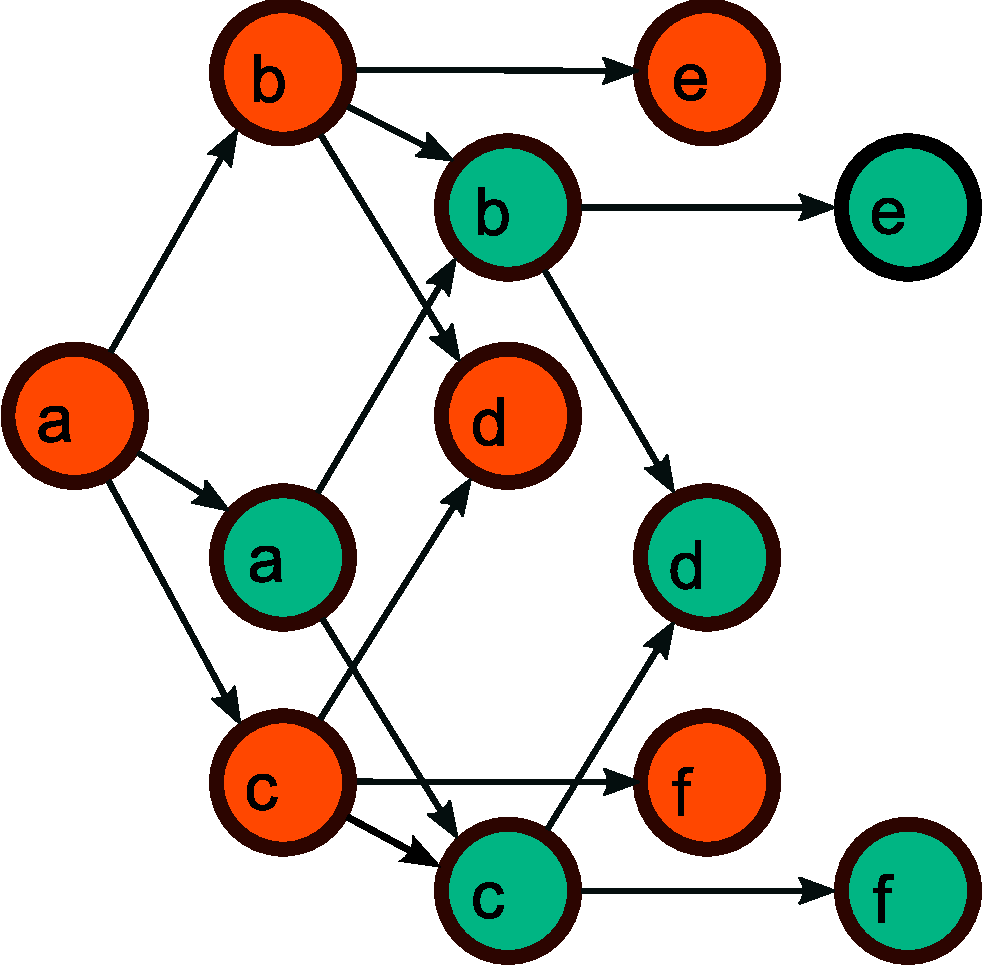
\includegraphics[width=6cm]{dependencies-two} \end{center}
    \caption{\small Complete dependency graph for the example
    system, assuming the least possible intercycle dependence: the
    forecast models ($a$, $b$, and $c$) depend on their own previous
    instances. The dashed arrows show connections to previous and
    subsequent forecast cycles.} 
    \label{fig-dep-two}
\end{figure}

As far as the author is aware existing forecast schedulers, in one
way or another, assume (and therefore require) a series of distinct
forecast cycles at all times. This fits with our intuitive view of
forecasting systems based on normal real time operations, and it means
the aforementioned nasty inter-cycle dependencies can be avoided. But
there is a cost to this simplification: strict seqential cycling is a
serious impediment when advance availability of external driving data
makes it possible, in principle, to run tasks from future cycles before
the current cycle is finished.  This occurs after delays (late arrival
of external data, system maintenance, etc.) and, to an even greater
extent, in historical case studies and parallel test systems that are
delayed with respect to the main operation. It is in fact a serious
problem for systems that have little downtime between forecast cycles
and consequently take many cycles to catch up after a delay. When
intercycle dependencies are ignored, the best that can be done in these
situations, in general, is to reduce the gap between cycles to zero. A
limited crude overlap of the single cycle job schedule may be possible
for specific task sets in certain circumstances, but even this is
sub-optimal and it would be very difficult to guarantee that no
dependencies will ever be violated.

\begin{figure} \begin{center}
    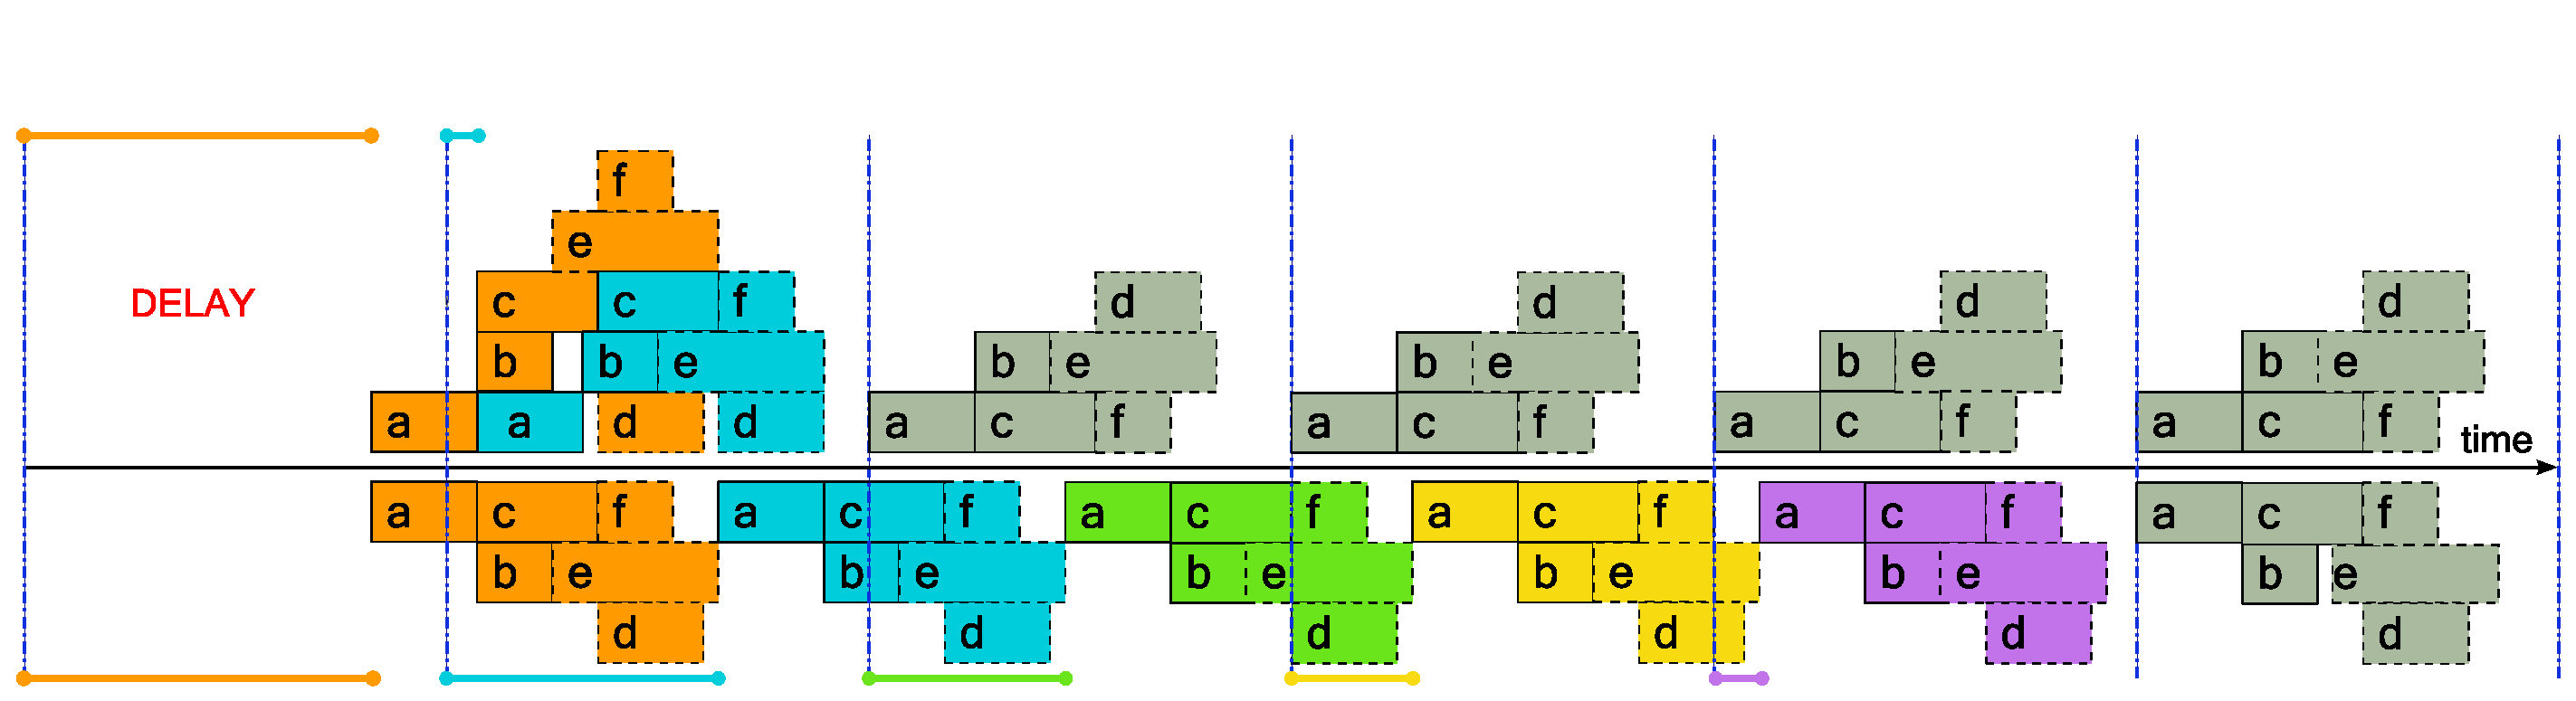
\includegraphics[width=12cm]{timeline-three} \end{center}
    \caption{\small Job schedules for the example system after a delay
    of almost one whole forecast cycle, when intercycle dependencies are
    taken into account (above the time axis), and when they are not
    (below the time time axis). The colored lines indicate the time that
    each cycle is delayed, and normal ``caught up'' cycles
    are shaded gray.} 
    \label{fig-time-three}
\end{figure} 
\begin{figure} 
    \begin{center} 
        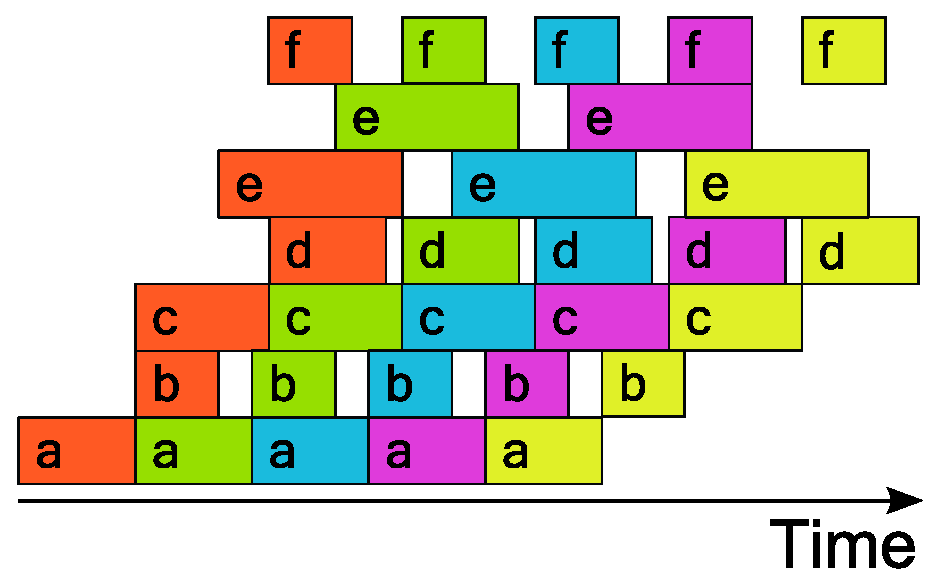
\includegraphics[width=8cm]{timeline-two}
    \end{center} 
    \caption{\small Job schedules for the example system in case study
    mode, or after a long delay, when the external driving data are
    available many cycles in advance. Above the time axis is the optimal
    schedule obtained when the system is constrained only by its true
    dependencies, as in Figure \ref{fig-dep-two}, and underneath is
    the best that can be done, in general, when intercycle dependencies
    are ignored.} 
    \label{fig-time-two}
\end{figure} 

Figure \ref{fig-time-three} shows the effect of an operational delay of
almost one whole cycle on a sequentially cycling system that has little
downtime between cycles - it takes many cycles to catch up. Above the
time axis is the optimal schedule that is possible, in principle, when
intercycle dependencies are taken into account: the second cycle after
the delay is hardly affected, and subsequent cycles are all on time.
Note that simply overlapping the single cycle schedules of Figure
\ref{fig-time-one} from the same start point would have resulted in
dependency violation by task {\em c}. Similarly, Figure
\ref{fig-time-two} shows job schedules for the example system in case
study mode, or when catching up after a very long delay, when the
external driving data are available many cycles in advance.  Task {\em
a}, which as the most upstream forecast model is likely to be a resource
intensive atmosphere or ocean model, has no dependence on cotemporal
tasks and can therefore run continuously, regardless of how much
downstream processing is yet to be completed in its own, or any
previous, forecast cycle. In practice task {\em a} would depend on
cotemporal upstream tasks that wait on the external driving data, but
they would return immediately when the external data is available in
advance, so the result stands. Other tasks can cycle at regular short
intervals, the interval depending on [CHECK THIS] the task run length
relative to that of its longest cotemporal upstream dependency path. In
this case {\em c} can also run continuously, and consecutive instances
of {\em e}, which has no previous-instance dependence, can overlap.
Thus, even for this very simple example system, tasks from three or four
different cycles can run simultaneously, in principle, at any given
time. 


\subsection{Existing Scheduling Systems}

As explained in the previous section, as far as the author is aware
current forecast scheduling systems ignore intercycle dependencies and
therefore require strict sequential cycle, which is very much
sub-optimal outside of normal real time operation. The simplest such
``scheduler'' places the burden of scheduling almost entirely on the
user, who must supply a list of tasks that the system will run through
sequence, perhaps with some way of specifying some crude functional
parallelism. This is clearly sub-optimal even for quite simple systems
and strict sequential cycling, and task ordering has to be re-evaluated
manually whenever the system is changed. 

Another method is system-specific finite state scheduling logic that
enforces a predetermined order of events: {\em if tasks A and B have
finished, then start task C} and so on. Optimal scheduling within a
forecast cycle is possible in this case but the hard coded logic
inevitably becomes convoluted and inflexible as system complexity
increases, and extension to intercycle dependencies is almost certainly
not feasible.  

Finally, the well established SMS system from ECMWF is an industrial
strength general scheduling tool for dependent jobs. Users define ``SMS
suites'' that group tasks into ``families'' and define explicit
dependency relationships. SMS does not appear to be able to do optimal
cycle-independent scheduling as shown in Figures~\ref{fig-time-one}
and~\ref{fig-time-two}, however, or at least is not able to do so when
configured for normal usage (THIS IS STILL NOT ENTIRELY RESOLVED!)
because it still relies on global cycling mechanisms to either loop
over successive forecast reference times or, for real time operation,
trigger off the wall clock.

\section{Cylc}

\subsection{Introduction}
Other systems cannot do optimal scheduling because they are unaware of
intercycle dependencies {\em and} they invariably use global forecast
cycle and/or date-time loops to advance the system forward in time,
which maintains the artificial boundary between cycles.  In contrast,
cylc has no system-wide looping mechansim: instead it maintains an
evolving pool of task proxy objects (representing the real tasks) each
of which has its own private cycle time and spawns its own successor
when it is ready (exactly when this is depends on task type; see
Section~\ref{sec:implementation}). Each task proxy knows its own
prerequisites (including those from previous cycles), but not who is
expected to provide them; and its own outputs, but not who is expected
to use them. It also knows how to invoke its external task once its
prerequisites are satisfied and, by means of a messaging system, can
record the external task's outputs as they are completed. Cylc then
gets the task pool to interact indiscriminately, {\em regardless of
cycle time}, to match unsatisfied prerequisites with completed
outputs.\footnote{In fact this negotiation goes through a middleman or
broker, which reduces the task interaction scaling from $n^2$ to $n$,
where $n$ is the number of tasks.} Thus optimal task scheduling emerges
naturally at run time, in all modes of operation.

Note that in addition to achieving optimal scheduling, this algorithm is
extremely simple. The entire forecasting system is defined by a simple
list of tasks each of which, in effect, thinks it is alone in the world
(even a standalone task must know its own prerequisites and
outputs).\footnote{You can still use explicit task dependence if you
wish: just make a task depend on an explicitly named upstream supplier
{\em finishing} rather than on the upstream output that is the actual
prerequisite of interest. However, framing prerequisites in terms of
required input filenames, or similar, results in a more flexible system:
tasks can easily be ``hot replaced'' by other tasks that generate
similar outputs for instance.}  For this to work, of course, the life
cycle of a task proxy object must be such that it is guaranteed to exist
by the time it is needed, but not too much earlier, and it should die
not too long after it is no longer needed.  This requires some thought
at the program design stage, but only once, and the complexities therein
are entirely hidden from the user. 


%In other words the task pool must include waiting tasks whose
%prerequisites may {\em soon} be satisfied (but preferably no waiting
%tasks whose prerequisites will not be satisfied for some time yet),
%tasks that are currently running, and finished tasks whose outputs
%could still be needed by any current or future waiting task (but
%preferably not any finished tasks whose output will no longer be needed
%by anyone). 


\subsection{Implementation}
\label{sec:implementation}

{\huge TO DO: update and insert external file implementation.tex}


\subsection{Usage}
\label{sec:usage}


\section{Introduction/Overview}

\section{How to Set Up a New System}

\section{How to Modify an Existing System}

\section{How to Start Up a System}

\section{How to Interact with a Running System}

\section{Command Reference}

\lstset{
language=,
xleftmargin=2em,
basicstyle=\tiny
}


\subsection{cylc}

This is the top level user interface to all cylc sub-commands.

{
\color{MidnightBlue}
\lstinputlisting{command-usage/cylc.txt}
}


\subsection{cylc server}

This is the scheduler program. Multiple instances of the server can run
at once, to control different forecasting systems (e.g. a main operation
and several parallel test systems), so long as each system is configured
with a different ``system name'' in its user config file (this
distinguishes the objects registered by the different systems in the
single Pyro nameserver).

{
\color{MidnightBlue}
\lstinputlisting{command-usage/cylc-server.txt}
}


\subsection{cylc control}

Remote control for running systems.

{
\color{MidnightBlue}
\lstinputlisting{command-usage/cylc-control.txt}
}


\subsection{System Monitor Commands}

\subsubsection{cylc monitor-all}
{
\color{MidnightBlue}
\lstinputlisting{command-usage/monitor-all.txt}
}


\subsubsection{cylc monitor-running}

{
\color{MidnightBlue}
\lstinputlisting{command-usage/monitor-running.txt}
}

\subsubsection{cylc monitor-dummies}

{
\color{MidnightBlue}
\lstinputlisting{command-usage/monitor-dummies.txt}
}


\subsubsection{cylc monitor-pyro-ns}

{
\color{MidnightBlue}
\lstinputlisting{command-usage/monitor-pyro-ns.txt}
}



\label{config}
\section{Task Definition Files}

A {\em Task Definition File} defines the properties of a cylc task:
name, valid run times, prerequisites and postrequisites, the task
control script used to invoke the task, etc.  A cylc utility,
\verb=task_generator.py= parses task definition files and auto-generates
Python code that defines the objects that represent each task within
cylc.

\subsection{Typical Example}

Most tasks have only cotemporal (same reference time) upstream and
downstream dependencies (recall that every task is implicitly dependent
on the previous instance of its own class, in cylc). The following
task definition file is sufficient to completely define such a task.
Different postrequisites can be specified depending on reference time. 

\lstset{language=sh, numbers=left}

{
\color{MidnightBlue}
\lstinputlisting{../sys/templates/example.def}
}

\subsection{Full Task Definition Template}

\lstset{language=sh, numbers=left}

{
\color{MidnightBlue}
\lstinputlisting{../sys/templates/full_template.def}
}

\subsection{More Complex Task Behaviour}

\textit{In EcoConnect: only streamflow and topnet}

For tasks that have non-cotemporal upstream dependencies and/or need to  
override task class methods to define new behaviour, the Python task
code must currently be written directly. 

\section{Task Messaging Mechanism}

Each external task must:

\begin{itemize}
\item report (to cylc) when the task has started
\item report when the task has finished
\item report when every other registered task postrequisite has
completed
\end{itemize}

(Technically, the `started' and `finished' messages are just
postrequisites too, but they are special in that every task
must have them).

In addition, tasks can optionally:

\begin{itemize}
\item report any arbitrary unregistered (i.e. non-postrequisite)
messages, for debugging, logging, or progress monitoring purposes.
\end{itemize}

All incoming messages are logged by cylc, but only postrequisite
messages can affect the state of other task objects.

Task messages don't necessarily have to originate from top level task
control scripts. It's a probably a good idea to do this if possible, but
lower level scripts that are invoked as the task runs can communicate
directly with cylc if necessary.

\section{wrapper}

A simple a simple wrapper script invoked by cylc reports task
startup, invokes the task, and reports task completion or failure. 


\label{usage}
\section{Usage}

All user-configurable parameters are set in \verb#config.py#. There is
one commandline option to force a restart from the state dump file
(which may have been edited) instead of the configured start time and
task list:

\lstset{language=sh}

{
\begin{lstlisting}
ecocontroller [-r]
Options:
    + most inputs should be configured in config.py
    + [-r] restart from the state dump file
\end{lstlisting}
}

\lstset{language=Python}

\subsection{Config File}

{
\color{MidnightBlue}
\lstinputlisting{../sys/examples/simple-0/user_config.py}
}



\appendix

\section{Essential OOP Concepts}

The cylc Python implementation makes heavy use of object oriented
programming concepts, particularly the {\em polymorphic} nature of
the task proxy objects.  This section contains a minimal introduction
to these Object Oriented Programming concepts.  Refer to any OOP
reference for more detail.

\subsection{Class}

A {\em class} is essentially a generalisation of {\em data type} to
include {\em behaviour} (i.e.\ functions or {\em methods}) as well as
state. For example, a $shape$ class could define a $position$ data
member that describes the location of each shape object, a $move()$
method that causes a shape object to alter its position, and a $draw()$
method that causes it to display itself in the right place on screen.

\subsection{Object}

{\em Objects} are more or less self contained specific {\em instances}
of a class. This is analagous to specific integer variables being 
instances of the general integer data type.

\subsection{Inheritance}

A {\em derived class} or {\em subclass} inherits the properties (methods
and data members) of a {\em base class}. It can also {\em override}
specific base class properties, or add new properties that aren't
present in the base class. Calling a particular method on an object
invokes the object's own class method if one is defined, otherwise the
immediate base class is searched, and so on down to the root of the
inheritance graph. 

For example, we could derive a $circle$ class from $shape$, adding a
`radius' data member and overriding the $draw()$ to get circle objects
to display themselves as actual circles.  Because we didn't override the
$move()$ method, calling $circle.move()$ would invoke the base class
method, $shape.move()$. 


\subsection{Polymorphism}

Polymorphism is the ability of one type to appear as and be used like
another type.  In OOP languages with inheritance, this usually refers to
the ability to treat derived/sub-class objects as if they were members
of a base class.  In particular, a group of mixed-type objects can all
be treated as members of a common base class. For example, we could
construct a list of $shape$ objects from $circles$, $triangles$, and
$squares$; calling $[list member].draw()$ will invoke the right derived
class $draw()$. This is a very powerful mechanism because {\em it allows
unmodified old code to call new code}: if we later derive an entirely
new kind of shape ($hexagon$, say) with it's own unique behaviour, the
existing program, without modification, will process the new objects in
the proper hexagon-specific way.  In Cylc, all task proxy objects are
derived from a common base class. The main algorithm works with
instances of the base class so that any current or future derived task
object can be handled by the program without modification (other than
the derived class code, that is).


\section{Threading in Pyro} \label{pyro-appendix}

With Pyro in {\em single threaded mode}, \verb#handleRequests()# returns
after {\em either} a timeout has occurred {\em or} at least one request
(i.e.\ remote method call) was handled. With \verb#timeout = None# this
allows us to process tasks {\em only} after remote method invocations
come in.  Further, we can detect the remote calls that actually change
task states, and thereby drop into the task processing code only when
necessary, which minimizes non-useful output from the task processing
loop (e.g.\ in dummy mode there are a lot of remote calls on the dummy
clock object, which does not alter tasks at all). 

In {\em multithreaded mode}, \verb#handleRequests()# returns immediately
after creating a new request handling thread for a single remote object,
and thereafter remote method calls on that object come in asynchronously
in the dedicated thread. This is not good for the dynamic scheduling
algorithm because tasks are only set running in the task processing
block which can be delayed while \verb#handleRequests()# blocks waiting
for a new connection to be established, even as messages that warrant
task processing are coming in on existing connections. The only way
around this seems to be to do task processing on \verb#handleRequests()#
timeouts which results in a lot of unnecessary processing when nothing
important is happening.


\section{Miscellaneous Notes}

\subsection{Orderly Product Generation}

Note that ``correct scheduling'' is not equivalent to ``orderly
generation of products by cycle time'' - under cylc a product
generation task will trigger as soon as its prerequisites are satisfied,
whether or not other tasks associated with the same cycle time are
running yet.  If your product delivery system demands that all products
for a given cycle time are uploaded at once then (a) fix it!, or (b)
you'll have to introduce artificial dependencies into your cylc system
to enforce strict sequential cycling (but that, of course, nullifies the
principal advantage of using cylc in the first place!)

\subsection{Catching Up}

The state of being ``caught up'' or not is a property of individual
tasks, not the whole system, and additionally it should only matter to
external contact tasks, i.e. those that wait on external data that is
available at a wall clock time of T (task cycle time) + o (some offset
insterval). Where this matters an external task can detect whether or
not it has caught up (and signal this to its proxy object in cylc) by
comparing its reference time (and offset) to the wall clock time.


\end{document}
